\documentclass{report}

\usepackage[T1]{fontenc}
\usepackage[utf8]{inputenc}
\usepackage[brazil]{babel}
%\usepackage[math]{anttor} % fonte um pouco mais estilizada
\everymath{\displaystyle}
\usepackage{import}
%\usepackage{parskip}
%=========================Packages==================================%
\usepackage{textcomp}
\usepackage{color,lscape, amsmath, hyperref, booktabs, latexsym, multicol, gensymb, lmodern, natbib, tikz, tkz-euclide, amssymb, enumitem, fancyhdr, lipsum, siunitx, setspace}
\usepackage{graphicx}

\newenvironment{Figure}
  {\par\medskip\noindent\minipage{\linewidth}}
  {\endminipage\par\medskip}

% configurações das questões, bem como: pontuação e estrutura.

\usepackage{tasks} % cria lista curta
\usepackage{exsheets} % cria questoes
\SetupExSheets[points]{name=ponto/s,number-format=\color{blue}} % define as configurações de pontuação das questões, e a cor da pontuação.

\DeclareInstance{exsheets-heading}{fancy-wp}{default}{
toc-reversed = true ,
indent-first = true ,
vscale = 2 ,
pre-code = \rule{\linewidth}{1pt} ,
post-code = \rule{\linewidth}{1pt} ,
title-format = \large\scshape\color{rgb:red,0.65;green,0.04;blue,0.07} ,
number-format = \large\bfseries\color{rgb:red,0.02;green,0.04;blue,0.48} ,
points-format = \itshape ,
points-pre-code = ( ,
points-post-code = ) ,
join =
{
number[r,B]title[l,B](.333em,0pt) ;
number[r,B]points[l,B](.333em,0pt)
} ,
attach = { main[hc,vc]number[hc,vc](0pt,0pt) }
}

%\SetupExSheets{headings=fancy-wp} % estilo diferente para o topo do enunciado com o nome " Exercício
%===========================Margins==============================%
\usepackage[top=8mm, bottom=20mm, left=8mm, right=8mm]{geometry}

%======================Cabeçalho e Rodapé========================%
\pagestyle{fancy}
\lfoot{\notaesquerda}
\cfoot{\thepage}
\rfoot{\notadireita}
%\lhead{HELLO}
%\chead{HELLO}
%\rhead{\textbf{The performance of new graduates}}
%\renewcommand{\headrulewidth}{0.4pt} %linha horizontal no topo da pagina
\renewcommand{\footrulewidth}{0.4pt} %linha horizontal no pé da pagina

\setlength\parindent{0pt}
\setlength\parskip{1.5ex}
\setlength\parsep{1.5\parskip}
%\thispagestyle{empty}%\bigskip %Rodapé na primeira pagina

\newcommand{\Qed}{\begin{flushright}\qed\end{flushright}}
\newcommand{\parinn}{\setlength{\parindent}{1cm}}
\newcommand{\parinf}{\setlength{\parindent}{0cm}}
\newcommand{\norm}{\|\cdot\|}
\newcommand{\inorm}{\norm_{\infty}}
\newcommand{\opensets}{\{V_{\alpha}\}_{\alpha\in I}}
\newcommand{\oset}{V_{\alpha}}
\newcommand{\opset}[1]{V_{\alpha_{#1}}}
\newcommand{\lub}{\text{lub}}
\newcommand{\del}[2]{\frac{\partial #1}{\partial #2}}
\newcommand{\Del}[3]{\frac{\partial^{#1} #2}{\partial^{#1} #3}}
\newcommand{\deld}[2]{\dfrac{\partial #1}{\partial #2}}
\newcommand{\Deld}[3]{\dfrac{\partial^{#1} #2}{\partial^{#1} #3}}
\newcommand{\uin}{\mathbin{\rotatebox[origin=c]{90}{$\in$}}}
\newcommand{\usubset}{\mathbin{\rotatebox[origin=c]{90}{$\subset$}}}
\newcommand{\lt}{\left}
\newcommand{\rt}{\right}
\newcommand{\bs}[1]{\boldsymbol{#1}}
\newcommand{\exs}{\exists}
\newcommand{\st}{\strut}
\newcommand{\dps}[1]{\displaystyle{#1}}

\newcommand{\sol}{\setlength{\parindent}{0cm}\textbf{\textit{Solution:}}\setlength{\parindent}{1cm} }
\newcommand{\solve}[1]{\setlength{\parindent}{0cm}\textbf{\textit{Solution: }}\setlength{\parindent}{1cm}#1 \Qed}
\newcommand{\mat}[1]{\left[\begin{matrix}#1\end{matrix}\right]}
\newcommand\numberthis{\addtocounter{equation}{1}\tag{\theequation}}

%---------------------------------------
% BlackBoard Math Fonts :-
%---------------------------------------

%Captital Letters
\newcommand{\bbA}{\mathbb{A}}	\newcommand{\bbB}{\mathbb{B}}
\newcommand{\bbC}{\mathbb{C}}	\newcommand{\bbD}{\mathbb{D}}
\newcommand{\bbE}{\mathbb{E}}	\newcommand{\bbF}{\mathbb{F}}
\newcommand{\bbG}{\mathbb{G}}	\newcommand{\bbH}{\mathbb{H}}
\newcommand{\bbI}{\mathbb{I}}	\newcommand{\bbJ}{\mathbb{J}}
\newcommand{\bbK}{\mathbb{K}}	\newcommand{\bbL}{\mathbb{L}}
\newcommand{\bbM}{\mathbb{M}}	\newcommand{\bbN}{\mathbb{N}}
\newcommand{\bbO}{\mathbb{O}}	\newcommand{\bbP}{\mathbb{P}}
\newcommand{\bbQ}{\mathbb{Q}}	\newcommand{\bbR}{\mathbb{R}}
\newcommand{\bbS}{\mathbb{S}}	\newcommand{\bbT}{\mathbb{T}}
\newcommand{\bbU}{\mathbb{U}}	\newcommand{\bbV}{\mathbb{V}}
\newcommand{\bbW}{\mathbb{W}}	\newcommand{\bbX}{\mathbb{X}}
\newcommand{\bbY}{\mathbb{Y}}	\newcommand{\bbZ}{\mathbb{Z}}

%---------------------------------------
% MathCal Fonts :-
%---------------------------------------

%Captital Letters
\newcommand{\mcA}{\mathcal{A}}	\newcommand{\mcB}{\mathcal{B}}
\newcommand{\mcC}{\mathcal{C}}	\newcommand{\mcD}{\mathcal{D}}
\newcommand{\mcE}{\mathcal{E}}	\newcommand{\mcF}{\mathcal{F}}
\newcommand{\mcG}{\mathcal{G}}	\newcommand{\mcH}{\mathcal{H}}
\newcommand{\mcI}{\mathcal{I}}	\newcommand{\mcJ}{\mathcal{J}}
\newcommand{\mcK}{\mathcal{K}}	\newcommand{\mcL}{\mathcal{L}}
\newcommand{\mcM}{\mathcal{M}}	\newcommand{\mcN}{\mathcal{N}}
\newcommand{\mcO}{\mathcal{O}}	\newcommand{\mcP}{\mathcal{P}}
\newcommand{\mcQ}{\mathcal{Q}}	\newcommand{\mcR}{\mathcal{R}}
\newcommand{\mcS}{\mathcal{S}}	\newcommand{\mcT}{\mathcal{T}}
\newcommand{\mcU}{\mathcal{U}}	\newcommand{\mcV}{\mathcal{V}}
\newcommand{\mcW}{\mathcal{W}}	\newcommand{\mcX}{\mathcal{X}}
\newcommand{\mcY}{\mathcal{Y}}	\newcommand{\mcZ}{\mathcal{Z}}



%---------------------------------------
% Bold Math Fonts :-
%---------------------------------------

%Captital Letters
\newcommand{\bmA}{\boldsymbol{A}}	\newcommand{\bmB}{\boldsymbol{B}}
\newcommand{\bmC}{\boldsymbol{C}}	\newcommand{\bmD}{\boldsymbol{D}}
\newcommand{\bmE}{\boldsymbol{E}}	\newcommand{\bmF}{\boldsymbol{F}}
\newcommand{\bmG}{\boldsymbol{G}}	\newcommand{\bmH}{\boldsymbol{H}}
\newcommand{\bmI}{\boldsymbol{I}}	\newcommand{\bmJ}{\boldsymbol{J}}
\newcommand{\bmK}{\boldsymbol{K}}	\newcommand{\bmL}{\boldsymbol{L}}
\newcommand{\bmM}{\boldsymbol{M}}	\newcommand{\bmN}{\boldsymbol{N}}
\newcommand{\bmO}{\boldsymbol{O}}	\newcommand{\bmP}{\boldsymbol{P}}
\newcommand{\bmQ}{\boldsymbol{Q}}	\newcommand{\bmR}{\boldsymbol{R}}
\newcommand{\bmS}{\boldsymbol{S}}	\newcommand{\bmT}{\boldsymbol{T}}
\newcommand{\bmU}{\boldsymbol{U}}	\newcommand{\bmV}{\boldsymbol{V}}
\newcommand{\bmW}{\boldsymbol{W}}	\newcommand{\bmX}{\boldsymbol{X}}
\newcommand{\bmY}{\boldsymbol{Y}}	\newcommand{\bmZ}{\boldsymbol{Z}}
%Small Letters
\newcommand{\bma}{\boldsymbol{a}}	\newcommand{\bmb}{\boldsymbol{b}}
\newcommand{\bmc}{\boldsymbol{c}}	\newcommand{\bmd}{\boldsymbol{d}}
\newcommand{\bme}{\boldsymbol{e}}	\newcommand{\bmf}{\boldsymbol{f}}
\newcommand{\bmg}{\boldsymbol{g}}	\newcommand{\bmh}{\boldsymbol{h}}
\newcommand{\bmi}{\boldsymbol{i}}	\newcommand{\bmj}{\boldsymbol{j}}
\newcommand{\bmk}{\boldsymbol{k}}	\newcommand{\bml}{\boldsymbol{l}}
\newcommand{\bmm}{\boldsymbol{m}}	\newcommand{\bmn}{\boldsymbol{n}}
\newcommand{\bmo}{\boldsymbol{o}}	\newcommand{\bmp}{\boldsymbol{p}}
\newcommand{\bmq}{\boldsymbol{q}}	\newcommand{\bmr}{\boldsymbol{r}}
\newcommand{\bms}{\boldsymbol{s}}	\newcommand{\bmt}{\boldsymbol{t}}
\newcommand{\bmu}{\boldsymbol{u}}	\newcommand{\bmv}{\boldsymbol{v}}
\newcommand{\bmw}{\boldsymbol{w}}	\newcommand{\bmx}{\boldsymbol{x}}
\newcommand{\bmy}{\boldsymbol{y}}	\newcommand{\bmz}{\boldsymbol{z}}

%---------------------------------------
% Scr Math Fonts :-
%---------------------------------------

\newcommand{\sA}{{\mathscr{A}}}   \newcommand{\sB}{{\mathscr{B}}}
\newcommand{\sC}{{\mathscr{C}}}   \newcommand{\sD}{{\mathscr{D}}}
\newcommand{\sE}{{\mathscr{E}}}   \newcommand{\sF}{{\mathscr{F}}}
\newcommand{\sG}{{\mathscr{G}}}   \newcommand{\sH}{{\mathscr{H}}}
\newcommand{\sI}{{\mathscr{I}}}   \newcommand{\sJ}{{\mathscr{J}}}
\newcommand{\sK}{{\mathscr{K}}}   \newcommand{\sL}{{\mathscr{L}}}
\newcommand{\sM}{{\mathscr{M}}}   \newcommand{\sN}{{\mathscr{N}}}
\newcommand{\sO}{{\mathscr{O}}}   \newcommand{\sP}{{\mathscr{P}}}
\newcommand{\sQ}{{\mathscr{Q}}}   \newcommand{\sR}{{\mathscr{R}}}
\newcommand{\sS}{{\mathscr{S}}}   \newcommand{\sT}{{\mathscr{T}}}
\newcommand{\sU}{{\mathscr{U}}}   \newcommand{\sV}{{\mathscr{V}}}
\newcommand{\sW}{{\mathscr{W}}}   \newcommand{\sX}{{\mathscr{X}}}
\newcommand{\sY}{{\mathscr{Y}}}   \newcommand{\sZ}{{\mathscr{Z}}}


%---------------------------------------
% Math Fraktur Font
%---------------------------------------

%Captital Letters
\newcommand{\mfA}{\mathfrak{A}}	\newcommand{\mfB}{\mathfrak{B}}
\newcommand{\mfC}{\mathfrak{C}}	\newcommand{\mfD}{\mathfrak{D}}
\newcommand{\mfE}{\mathfrak{E}}	\newcommand{\mfF}{\mathfrak{F}}
\newcommand{\mfG}{\mathfrak{G}}	\newcommand{\mfH}{\mathfrak{H}}
\newcommand{\mfI}{\mathfrak{I}}	\newcommand{\mfJ}{\mathfrak{J}}
\newcommand{\mfK}{\mathfrak{K}}	\newcommand{\mfL}{\mathfrak{L}}
\newcommand{\mfM}{\mathfrak{M}}	\newcommand{\mfN}{\mathfrak{N}}
\newcommand{\mfO}{\mathfrak{O}}	\newcommand{\mfP}{\mathfrak{P}}
\newcommand{\mfQ}{\mathfrak{Q}}	\newcommand{\mfR}{\mathfrak{R}}
\newcommand{\mfS}{\mathfrak{S}}	\newcommand{\mfT}{\mathfrak{T}}
\newcommand{\mfU}{\mathfrak{U}}	\newcommand{\mfV}{\mathfrak{V}}
\newcommand{\mfW}{\mathfrak{W}}	\newcommand{\mfX}{\mathfrak{X}}
\newcommand{\mfY}{\mathfrak{Y}}	\newcommand{\mfZ}{\mathfrak{Z}}
%Small Letters
\newcommand{\mfa}{\mathfrak{a}}	\newcommand{\mfb}{\mathfrak{b}}
\newcommand{\mfc}{\mathfrak{c}}	\newcommand{\mfd}{\mathfrak{d}}
\newcommand{\mfe}{\mathfrak{e}}	\newcommand{\mff}{\mathfrak{f}}
\newcommand{\mfg}{\mathfrak{g}}	\newcommand{\mfh}{\mathfrak{h}}
\newcommand{\mfi}{\mathfrak{i}}	\newcommand{\mfj}{\mathfrak{j}}
\newcommand{\mfk}{\mathfrak{k}}	\newcommand{\mfl}{\mathfrak{l}}
\newcommand{\mfm}{\mathfrak{m}}	\newcommand{\mfn}{\mathfrak{n}}
\newcommand{\mfo}{\mathfrak{o}}	\newcommand{\mfp}{\mathfrak{p}}
\newcommand{\mfq}{\mathfrak{q}}	\newcommand{\mfr}{\mathfrak{r}}
\newcommand{\mfs}{\mathfrak{s}}	\newcommand{\mft}{\mathfrak{t}}
\newcommand{\mfu}{\mathfrak{u}}	\newcommand{\mfv}{\mathfrak{v}}
\newcommand{\mfw}{\mathfrak{w}}	\newcommand{\mfx}{\mathfrak{x}}
\newcommand{\mfy}{\mathfrak{y}}	\newcommand{\mfz}{\mathfrak{z}}

%---------------------------------------
% Bar
%---------------------------------------

%Captital Letters
\newcommand{\barA}{\overline{A}}	\newcommand{\barB}{\overline{B}}
\newcommand{\barC}{\overline{C}}	\newcommand{\barD}{\overline{D}}
\newcommand{\barE}{\overline{E}}	\newcommand{\barF}{\overline{F}}
\newcommand{\barG}{\overline{G}}	\newcommand{\barH}{\overline{H}}
\newcommand{\barI}{\overline{I}}	\newcommand{\barJ}{\overline{J}}
\newcommand{\barK}{\overline{K}}	\newcommand{\barL}{\overline{L}}
\newcommand{\barM}{\overline{M}}	\newcommand{\barN}{\overline{N}}
\newcommand{\barO}{\overline{O}}	\newcommand{\barP}{\overline{P}}
\newcommand{\barQ}{\overline{Q}}	\newcommand{\barR}{\overline{R}}
\newcommand{\barS}{\overline{S}}	\newcommand{\barT}{\overline{T}}
\newcommand{\barU}{\overline{U}}	\newcommand{\barV}{\overline{V}}
\newcommand{\barW}{\overline{W}}	\newcommand{\barX}{\overline{X}}
\newcommand{\barY}{\overline{Y}}	\newcommand{\barZ}{\overline{Z}}
%Small Letters
\newcommand{\bara}{\overline{a}}	\newcommand{\barb}{\overline{b}}
\newcommand{\barc}{\overline{c}}	\newcommand{\bard}{\overline{d}}
\newcommand{\bare}{\overline{e}}	\newcommand{\barf}{\overline{f}}
\newcommand{\barg}{\overline{g}}	\newcommand{\barh}{\overline{h}}
\newcommand{\bari}{\overline{i}}	\newcommand{\barj}{\overline{j}}
\newcommand{\bark}{\overline{k}}	\newcommand{\barl}{\overline{l}}
\newcommand{\barm}{\overline{m}}	\newcommand{\barn}{\overline{n}}
\newcommand{\baro}{\overline{o}}	\newcommand{\barp}{\overline{p}}
\newcommand{\barq}{\overline{q}}	\newcommand{\barr}{\overline{r}}
\newcommand{\bars}{\overline{s}}	\newcommand{\bart}{\overline{t}}
\newcommand{\baru}{\overline{u}}	\newcommand{\barv}{\overline{v}}
\newcommand{\barw}{\overline{w}}	\newcommand{\barx}{\overline{x}}
\newcommand{\bary}{\overline{y}}	\newcommand{\barz}{\overline{z}}

%---------------------------------------
% Greek Letters:-
%---------------------------------------
\newcommand{\eps}{\epsilon}
\newcommand{\veps}{\varepsilon}
\newcommand{\lm}{\lambda}
\newcommand{\Lm}{\Lambda}
\newcommand{\gm}{\gamma}
\newcommand{\Gm}{\Gamma}
\newcommand{\vph}{\varphi}
\newcommand{\ph}{\phi}
%\newcommand{\th}{\theta}


\title{\Huge{Analysis 2 Lecture Notes}\\ \hspace{4cm}-- Upendra Kulkarni}
\author{\huge{Soham Chatterjee}}
\date{}

\global\hbadness=1199
\global\hbadness=4531
\DeclareFontShape{OT1}{cmr}{bx}{sc}{<-> cmbcsc10}{}



\begin{document}
\thispagestyle{empty}
\mytitleb{Matrizes}{Fernando Jorge}{}{2023}
\newpage% or \cleardoublepage
\vspace*{5cm}

\begin{center}
	\textbf{Introduction}
\end{center}

This is the lecture notes scribed by me. If you find any mistakes in the notes please email me at \url{sohamc@cmi.ac.in}. 

The whole course is taken by Prof. Upendra Kulkarni, online. If you want the lecture videos then you can find them in \href{https://youtube.com/playlist?list=PL8I7rVYxS9smyQemVlU10yF9F37ZQN38P}{this link}. Sir mainly followed Prof. Pramath Sastry's Notes (\url{https://www.cmi.ac.in/~pramath/teaching.html#ANA2}). You can find all the assignments problems in the following  \href{https://drive.google.com/drive/folders/1dODMladIJ1f4BfMXVxoU5_YkfmWU8v4q?usp=share_link}{drive link}. Through out the course the book we followed is  Principles of Mathematical Analysis by Walter Rudin. 
\pagebreak

% \pdfbookmark[<level>]{<title>}{<dest>}
\pdfbookmark[section]{\contentsname}{toc}
\tableofcontents
\pagebreak

\chapter{Introdução}

Observe abaixo a tabela da expectativa de vida no Brasil em 2008, segundo as regiões brasileiras (numeradas de 1 a 5) e gêneros (1 e 2). 

\begin{figure}[htb!]
  \centering
  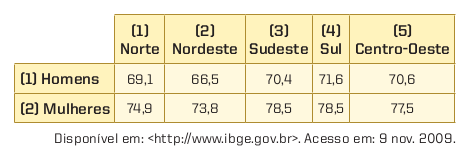
\includegraphics[width=.6\linewidth]{images/quadro.png}
  \caption{expectativa de vida brasileira em 2008}
  \label{fig:}
\end{figure}

Note que podemos encontrar a expectativa de vida de uma mulher residente na região Sul bastando olhar o cruzamento da linha 2 com a coluna 4, onde encontramos o valor de 78,5 anos. 

Em matemática, as tabelas como essa são chamadas de \textbf{matrizes}, sobre as quais definiremos a relação de igualdade e algumas operações. 


\section{Definição}
\dfn{Matriz}{Chama-se \textbf{matriz do tipo $m \times n$} (lemos ``m por n'') toda tabela de números dispostos em \textit{m} linhas e \textit{n} colunas.
} 

\begin{note}
  Essa tabela deve ser representada entre parênteses () ou entre colchetes [].
\end{note}

\ex{}{

  \begin{tasks}
    \task{
      $\begin{bmatrix}
        -6 & 7 \\
        -4 & 0 \\
        2 & -1 \\
      \end{bmatrix}$ 
      é uma matriz do tipo $3 \times 2$, pois tem 3 linhas e 2 colunas.
    }
    \task {
    $\begin{bmatrix}
      3 & \sqrt{2} & -5
    \end{bmatrix}$
    é uma matriz do tipo $1 \times 3$, pois tem 1 linha e 3 colunas.
    }
  \end{tasks}
}

\section{Representação genérica}

Indicamos por \textbf{$a_{ij}$} o elemento posicionado na linha \textit{i} e na coluna \textit{j} de uma matriz \textit{A}.

\ex{}{
  Na matriz:

  \begin{equation*}
    A_{3 \times 2} = \begin{bmatrix}
      6 & 7 \\
      -4 & 0 \\
      2 & -1
    \end{bmatrix}
  \end{equation*}

  \begin{itemize}
    \item o elemento 6 está na linha 1 e na coluna 1; por isso, ele é indicado por $a_{11}$, ou seja, $a_{11} = 6$;
    \item o elemento 7 está na linha 1 e na coluna 2; por isso, ele é indicado por $a_{12}$, ou seja, $a_{12} = 7$;
    \item analogamente, temos $a_{21} = -4$, $a_{22} = 0$, $a_{31} = 2$, $a_{32} = -1$.
  \end{itemize}


}

\dfn{Matriz Genérica}{
  Representamos genericamente uma matriz \textit{A} do tipo $m \times n$ da seguinte maneira:

  \begin{equation*}
    A_{m \times n} = \begin{bmatrix}
      a_{11} & a_{12} & a_{13} & \dots & a_{1n} \\
      a_{21} & a_{22} & a_{23} & \dots & a_{2n} \\
      \vdots & \vdots & \vdots & \vdots & \vdots \\
      a_{m1} & a_{m2} & a_{m3} & \dots & a_{mn} \\
    \end{bmatrix}
  \end{equation*}
}
  Como essa representação é muita extensa, vamos convencionar uma forma abreviada. Essa matriz pode ser representada simplesmente por 
  $A = (a_{ij})_{m \times n}$ ou, quando não houver possibilidade de confusão quanto ao tipo de matriz, por $A = (a_{ij})$.

\qs{}{Representar explicitamente a matriz $A = (a_{ij})_{2 \times 4}$ tal que $a_{ij} = 2i + j$.}

\sol{Primeiro, representamos genericamente a matriz \textit{A}, do tipo $2 \times 4$:
  \begin{equation*}
    A = \begin{bmatrix}
      a_{11} & a_{12} & a_{13} & a_{14} \\
      a_{21} & a_{22} & a_{23} & a_{24} \\
    \end{bmatrix}
  \end{equation*}

  A seguir, calculamos o valor de cada elemento $a_{ij}$, pela lei $a_{ij} = 2i + j$:

  \begin{tasks}(2)
    \task[] $a_{11} = 2 \cdot 1 + 1 = 3$
    \task[] $a_{12} = 2 \cdot 1 + 2 = 4$
    \task[] $a_{13} = 2 \cdot 1 + 3 = 5$
    \task[] $a_{14} = 2 \cdot 1 + 4 = 6$
    \task[] $a_{21} = 2 \cdot 2 + 1 = 5$
    \task[] $a_{22} = 2 \cdot 2 + 2 = 6$
    \task[] $a_{23} = 2 \cdot 2 + 3 = 7$
    \task[] $a_{24} = 2 \cdot 2 + 4 = 8$
  \end{tasks}

  Concluindo, temos a matriz: $A = \begin{bmatrix}
    3 & 4 & 5 & 6 \\
    5 & 6 & 7 & 8
  \end{bmatrix}$
}

\section{Matrizes Especiais}

\subsection{Matriz Quadrada}

\dfn{Matriz Quadrada}{É toda matriz cujo número de linhas é igual ao número de colunas.}

\begin{note}
  O número de linhas ou de colunas de uma matriz quadrada é chamado de \textbf{ordem} da matriz.
\end{note}

\ex{}{

  \begin{tasks}
    \task $\begin{bmatrix}
      4 & 9 & 0 \\
      -6 & 2 & 4 \\
      3 & 5 & -2
    \end{bmatrix}$
    é uma matriz quadrada de ordem 3.

    \task $\begin{bmatrix}
      3 & -9 \\
      0 & 1
    \end{bmatrix}$
    é uma matriz quadrada de ordem 2.
  \end{tasks}
}

Numa matriz A de ordem \textit{n}, os elementos $a_{ij}$, tais que $i = j$ formam a \textbf{diagonal principal} da matriz, e os elementos 
$a_{ij}$, tais que $i + j = n + 1$ formam a \textbf{diagonal secundária}. Por exemplo:

\begin{figure}[htb!]
  \centering
  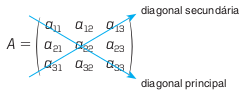
\includegraphics[width=.3\linewidth]{images/quadrada.png}
\end{figure}

\subsection{Matriz Identidade}

\dfn{Matriz Identidade}{É a matriz quadrada cujos elementos da \textbf{diagonal principal} são iguais a 1 e os demais iguais a 0.}

Indicamos por $I_n$ a matriz identidade de ordem \textit{n}.

\ex{}{
  \begin{tasks}
    \task $I_3 = \begin{bmatrix}
      1 & 0 & 0 \\
      0 & 1 & 0 \\
      0 & 0 & 1
    \end{bmatrix}$

    \task $I_2 = \begin{bmatrix}
      1 & 0 \\
      0 & 1
    \end{bmatrix}$
  \end{tasks}
}

\subsection{Matriz Nula}

\dfn{Matriz Nula}{É a matriz que possui todos os elementos iguais a zero.}

\ex{}{
  \begin{tasks}
    \task 
  $\begin{bmatrix}
    0 & 0 & 0 \\
    0 & 0 & 0 \\
    0 & 0 & 0 \\
  \end{bmatrix}$
  \task $\begin{bmatrix}
    0 & 0 \\
    0 & 0 \\
  \end{bmatrix}$
  \end{tasks}
}

\subsection{Transposta de uma Matriz}

\dfn{Transposta de uma Matriz}{Transposta de uma matriz \textit{A} é a matriz $A^t$ tal que os números que a formam são obtidos através da troca de posição entre linhas e colunas da matriz \textit{A}. }



\end{document}
